\chapter{basic}

\section{Mechine Learning}
\begin{itemize}
    \item supervised learning
    \item semi-supervised learning
    \item unsupervised learning
    \item reinforcement learning
    \item active learning
\end{itemize}

\section{iid}

\section{最小方差无偏估计}

\section{Maximum likelihood estimation}
深度学习来就是用模型$p_{model}(\boldsymbol{x};\boldsymbol{\theta})$来估计数据的真实分布$p_{data}(\boldsymbol{x};\boldsymbol{\theta})$,
对于一组确定的数据集$X$,在样本已被观察到的情况下,需要找到使得$p_{model}(X; \boldsymbol{\theta})$出现可能性最大的一组参数$\boldsymbol{\theta}$,也就是
最大似然估计:
\begin{equation}
    \begin{split}
        \boldsymbol{\theta}_{ML} &= \arg \max_\theta p_{model}(X, \boldsymbol{\theta}) \\
        &= \arg \max_{\boldsymbol{\theta}} \prod _{i=1}^m p_{model}(\boldsymbol{x}^i; \boldsymbol{\theta})
    \end{split}
\end{equation}
等价于
\begin{equation}
    \begin{split}
        \boldsymbol{\theta}_{ML} &= \arg \max_{\boldsymbol{\theta}} \sum_{i=0}^m \log p_{model}(\boldsymbol{x}^i; \boldsymbol{\theta})
    \end{split}
\end{equation}
除$m$,等价于
\begin{equation}
    \begin{split}
        \boldsymbol{\theta}_{ML} &= \arg \max_{\boldsymbol{\theta}} E _{x \sim \hat p_{data}} \log p_{model}(\boldsymbol{x}^i; \boldsymbol{\theta})
    \end{split}
\end{equation}

\subsection{KL divergence}
KL散度用来衡量两种分布之间的差异,
\begin{equation}
    \begin{split}
        D_{KL}(\hat p_{data}|| p_{model}) &= \int_{-\infty}^{+\infty} \hat p_{data}(\boldsymbol{x}) \ln{\frac{\hat p_{data}(\boldsymbol{x})}{p_{model}(\boldsymbol{x})}} \mathrm{d}x
    \end{split}
\end{equation}
$\hat p_{data}(\boldsymbol{x})$与模型无关

\section{Initialization scheme}
\subsection{constant initialization}

\subsection{random initialization}
按照某一分布随机初始化
\subsubsection{normal initialization}
\begin{equation}
    W \sim N(\mu, \sigma^2)
\end{equation}

\subsubsection{uniform initalization}
\begin{equation}
    W \sim U[-\frac{1}{\sqrt{n}}, \frac{1}{\sqrt{n}}]
\end{equation}

\subsection{xavier initalization}
针对使用\textbf{对称激活函数}$\tanh(x)$的网络进行参数初始化,对于ReLU激活函数并不适用\cite{Glorot2010}.

\subsubsection{Forward}
对于一个卷积层来说
\begin{equation}
    \begin{split}
        \mathbf{y}_l &= \mathbf{W}_l \mathbf{x}_l + \mathbf{b}_l\\
        \mathbf{x}_l &= f(\mathbf{y}_{l-1})
    \end{split}
\end{equation}
在如下前提和假设下
\begin{itemize}
    \item 初始化$\mathbf{W}_l$元素为独立同分布
    \item 假设$\mathbf{x}_l$元素也为独立同分布
    \item $\mathbf{w}_l$, $\mathbf{x}_l$互相独立
\end{itemize}
则有
\begin{equation}
    \begin{split}
        Var(\mathbf{y}_l) &= Var(\sum \mathbf{w}_l \mathbf{x}_l + \mathbf{b}_l)\\
        &= Var(\sum \mathbf{w}_l \mathbf{x}_l) \\
        &= n_l Var(\mathbf{w}_l \mathbf{x}_l)
    \end{split}
\end{equation}
令$\mathbf{w}_l$期望为0,$E(\mathbf{w}_l) = 0, Var(\mathbf{w}_l) = E(\mathbf{w}_l - E(\mathbf{w}_l))^2 = E\mathbf{w}_l^2$,则
\begin{equation}
    \begin{split}
        Var(\mathbf{y}_l) &= n_l E(\mathbf{w}_l^2\mathbf{x}_l^2) - n_l E^2\mathbf{w}_l E^2 \mathbf{x}_l \\
        &= n_l E(\mathbf{w}_l^2\mathbf{x}_l^2) \\
        &= n_l Var(\mathbf{w}_l)E(\mathbf{x}_l^2)
    \end{split}
\end{equation}
若$E\mathbf{x}_l = 0$,则
\begin{equation}
    Var(\mathbf{y}_l) = n_l Var(\mathbf{w}_l)Var(\mathbf{x}_l)
\end{equation}

若要实现$Var(\mathbf{y}_l) = Var(\mathbf{x}_l)$,则需要满足$n_l Var(\mathbf{w}_l) = 1$,即
\begin{equation}
    Var(\mathbf{w}_l) = \frac{1}{n_l}
\end{equation}

\begin{itemize}
    \item 若$\mathbf{w}_l$服从正态分布,则$\mathbf{w}_l \sim N(0, \frac{1}{n_l})$
    \item 若$\mathbf{w}_l$服从均匀分布,则$\mathbf{w}_l \sim U(-\sqrt{\frac{3}{n_l}}, \sqrt{\frac{3}{n_l}})$
\end{itemize}

\subsubsection{Backword}
反向传播过程中,需要保证梯度的方差不变,每一层的梯度为:
\begin{equation}
    \Delta \mathbf{x}_l = \hat{\mathbf{W}}_l \Delta \mathbf{y}_l
\end{equation}
假设
\begin{itemize}
    \item $\mathbf{w}_l$和$\Delta{\mathbf{y}}_l$互相独立
    \item $E\mathbf{w}_l = 0, E\Delta{\mathbf{x}}_l = 0$
\end{itemize}
同前向传播,可得
\begin{equation}
    \begin{split}
        Var(\Delta{\mathbf{x}_l}) &= \hat n_l Var(\mathbf{w}_l)Var(\Delta{\mathbf{y}}_l)
    \end{split}
\end{equation}
\begin{itemize}
    \item 若$\mathbf{w}_l$服从正态分布, 则$\mathbf{w}_l \sim N(0, \frac{1}{\hat n_l})$
    \item 若$\mathbf{w}_l$服从均匀分布,则$\mathbf{w}_l \sim U(-\sqrt{\frac{3}{\hat n_l}}, \sqrt{\frac{3}{\hat n_l}})$
\end{itemize}

除非$n = \hat n_l$,否则同时保证信号在向前向后传播时的Var不变,取调和平均数,$Var(\mathbf{w}_l) = \frac{2}{n_l + \hat n_l}$,可得
\begin{itemize}
    \item Normal distribution: $\mathbf{w}_l \sim N(0, \frac{2}{n_l + \hat n_l})$
    \item Uniform distribution: $\mathbf{w}_l \sim U(-\sqrt{\frac{6}{n_l+\hat n_l}}, \sqrt{\frac{6}{n_l+\hat n_l}})$
\end{itemize}


\subsection{orthogonal initalization}

\subsection{kaiming initalization}
Xavier 针对对称激活函数的层权重初始化进行设计,但对于使用ReLu激活函数的层并不适用。\\
对ReLU层来说,$E(\mathbf{x}_l^2) = \frac{1}{2}Var(\mathbf{y}_l)$,因此
\begin{equation}
    \begin{split}
        Var(\mathbf{y}_l) &= \frac{1}{2} n_l Var(\mathbf{w}_l)Var(\mathbf{x}_l) \\
        Var(\Delta{\mathbf{x}_l}) &= \frac{1}{2} \hat n_l Var(\mathbf{w}_l)Var(\Delta{\mathbf{y}}_l)
    \end{split}
\end{equation}
且在权重初始化时,使用上述任意一个即可。

\section{正则化}

\section{Data proprocessing}
\subsection{whitening}

\section{Activation functions}
\subsection{sigmoid}
\begin{tikzpicture}[domain=-2:2]
    \draw[very thin,color=gray] (-1.9, -1.9) grid (1.9, 1.9);
    \draw[->] (-2,0) -- (2,0) node[right] {$x$};
    \draw[->] (0,-2) -- (0,2) node[above] {$f(x)$};
    \draw[color=red]	plot (\x, { 1 / (1 + exp(-\x)) })   	node[right] {$g(x) = \frac{1}{1 + \mathrm{e^{-x}}}$};
\end{tikzpicture}

\begin{equation}
    \begin{split}
        g(x) &= \frac{1}{1+\mathrm{e}^{-x}} \\
        g(x)' &= g(x)(1-g(x))
    \end{split}
\end{equation}

\subsection{tanh(x)}
\begin{tikzpicture}[domain=-2:2]
    \draw[very thin,color=gray] (-1.9, -1.9) grid (1.9, 1.9);
    \draw[->] (-2,0) -- (2,0) node[right] {$x$};
    \draw[->] (0,-2) -- (0,2) node[above] {$f(x)$};
    \draw[color=blue]	plot (\x,{tanh(\x)})					node[right] {$g(x) = \tanh(x)$};
\end{tikzpicture}

\begin{equation}
    \begin{split}
        g(x) &= tanh(x) \\
        g(x)' &= 1 - g(x)^2 \\ &= 1 - \tanh(x)^2
    \end{split}
\end{equation}

\subsection{Rectified linear units}
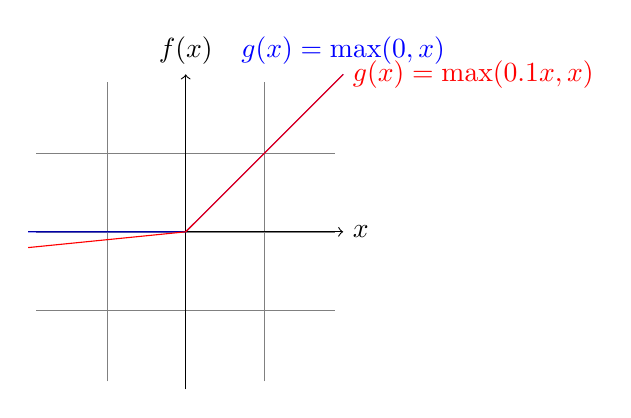
\begin{tikzpicture}[domain=-2:2]
    \draw[very thin,color=gray] (-1.9, -1.9) grid (1.9, 1.9);
    \draw[->] (-2,0) -- (2,0) node[right] {$x$};
    \draw[->] (0,-2) -- (0,2) node[above] {$f(x)$};
    \draw[color=blue]	plot (\x,{max(0, \x)})					node[above] {$g(x) = \max(0, x)$};
    \draw[color=red]	plot (\x,{max(0.1 * \x, \x)})			node[right] {$g(x) = \max(0.1x, x)$};
\end{tikzpicture}

\subsubsection{ReLU}
\begin{equation}
    g(x) = \max(0, x)
\end{equation}

\subsubsection{Leaky ReLU}
\begin{equation}
    g(x) = \max(0.01x, x)
\end{equation}

\subsubsection{PReLU}
\begin{equation}
    g(x) = \max(\alpha x, x)
\end{equation}

\subsection{haha}
\begin{tikzpicture}[domain=-2:2]
    \draw[very thin,color=gray] (-1.9, -1.9) grid (1.9, 1.9);
    \draw[->] (-2,0) -- (2,0) node[right] {$x$};
    \draw[->] (0,-2) -- (0,2) node[above] {$f(x)$};
    \draw[color=blue]	plot (\x,{tanh(\x) + 0.25 * \x})					node[right] {$g(x) = \tanh(x) + 0.25x$};
\end{tikzpicture}

\begin{equation}
    \begin{split}
        g(x) &= \tanh(x) + 0.25x \\
        g(x)' &= 0.75 - g(x)^2 \\ &= 0.75 - \tanh(x)^2
    \end{split}
\end{equation}

\subsection{Loss functions}

